\chapter{Development}

% Say this chapter turns the background claim into an empirical pipeline.
% State that the goal is to show emotion is recoverable and steerable in residual-space representations. 

This chapter translates the conceptual claims of the previous chapter into an empirical pipeline.\par
Our central objective is to test whether emotion can be recovered and steered in residual-space representations of a frozen language model. To achieve this, we progress from controlled data construction and residual-stream extraction to layer diagnostics, linear decodability analysis and causal steering via activation-space directions. We then examine the latent geometry that underpins these processes and evaluate whether steering can produce directional, monotonic affective change while preserving semantic content. In short, this chapter not only asks whether emotion is represented in hidden states, but also whether this representation can be used to control emotional editing.\par

\section{Dataset Construction}

In order to investigate whether emotion is encoded as structured geometry in residual space, we constructed controlled rewrite datasets from shared source utterances. The primary dataset is an emotion-category rewrite set derived from two dialogue corpora: DailyDialog~\cite{li2017dailydialogmanuallylabelledmultiturn} and EmpatheticDialogues~\cite{rashkin2019empatheticopendomainconversationmodels}. We selected dialogue data because conversational utterances provide compact emotional signals grounded in context in everyday interpersonal situations, while keeping propositional content sufficiently constrained for controlled rewriting. For each source utterance, we used GPT-4.1-mini to generate rewrites for Plutchik's eight basic emotions (joy, trust, fear, surprise, sadness, disgust, anger and anticipation) at three matched intensity levels (low, medium and high). This yields $8\times3 = 24$ affective variants per source text. A central constraint throughout the construction process was to preserve meaning: the underlying situation and factual content were held constant while only the affective framing was systematically varied.

\begin{table}[H]
\centering
\small
\begin{tabular}{p{0.12\linewidth} p{0.82\linewidth}}
\toprule
\textbf{Emotion} & \textbf{Utterance} \\
\midrule
\textbf{Base} & \textbf{I waited for hours and nobody came.} \\
Joy & Nobody came for hours, but I ended up enjoying the quiet time on my own. \\
Trust & Nobody came for hours, but I am sure they had a valid reason. \\
Fear & Nobody came for hours, and I started worrying that something might have gone wrong. \\
Surprise & Nobody came for hours, and honestly I did not expect that at all. \\
Sadness & For hours, nobody came. I guess that says enough. \\
Disgust & Nobody came for hours; that felt deeply inconsiderate. \\
Anger & Nobody came for hours, and I am really frustrated about wasting all that time. \\
Anticipation & Nobody came for hours, but I kept thinking they might still arrive any minute. \\
\bottomrule
\end{tabular}
\caption{Illustrative rewrites for all eight Plutchik emotion categories at matched medium intensity.}
\label{tab:emotion_rewrite_example}
\end{table}

As a control condition, we constructed an additional neutral paraphrase baseline dataset. In this dataset, each source utterance has been rewritten into an affectively neutral but semantically equivalent form. This baseline provides a reference representation of content without targeted emotional colouring, enabling contrastive analysis between emotion-conditioned and emotion-suppressed activations. \par

\begin{table}[H]
\centering
\small
\begin{tabular}{p{0.22\linewidth} p{0.72\linewidth}}
\toprule
\textbf{Field} & \textbf{Example} \\
\midrule
Base utterance & I waited for hours and nobody came. \\
Neutral paraphrase & I waited for several hours, and no one arrived. \\
Purpose & Preserve events and meaning while removing affective phrasing. \\
\bottomrule
\end{tabular}
\caption{Illustrative example from the neutral-paraphrase control dataset.}
\label{tab:neutral_rewrite_example}
\end{table}

Together, these datasets enable us to distinguish emotional signals from lexical-semantic content. This provides an empirical basis for the decodability, geometry and steering analyses presented in subsequent sections.\par

This design makes it possible to ask whether affective variation forms a consistent direction in activation space, rather than merely reflecting surface-level lexical differences between emotional words.\par

\section{Residual-Stream Extraction}

We extract hidden-state activations from a frozen, instruction-tuned language model (Llama-3.1-8B~\cite{meta2024llama318b}) with no gradient updates. Our aim is to determine where affective information is represented in the model's internal computations rather than in output tokens alone. The residual stream is therefore used as the primary analysis target because it is the shared channel through which each transformer block accumulates and propagates semantic and affective information across layers.

To ensure that the inputs are comparable across the different conditions, each sample is formatted with a shared instruction prefix that is constructed from the same base utterance. Only the continuation text is changed, either through an emotion rewrite or a neutral paraphrase. Specifically, we use a user instruction in the form of a chat template that asks for a rewrite aligned with the speaker's feelings, and then append the rewritten sentence as the assistant continuation. This matching protocol controls for variance at the prompt level and enables direct comparison of emotion-conditioned and neutral-conditioned activations.

\begin{table}[H]
\centering
\label{tab:activation_prompt}
\begin{tabular}{p{0.95\linewidth}}
\toprule
\textbf{Template Prompt} \\
\midrule
Please rewrite this so it aligns with my feelings more. \\
Start straight from the rewritten text without any preamble, and only provide \textbf{one} rewritten version. \\
Base: \texttt{\{base\_text\}} \\
\bottomrule
\end{tabular}
\caption{Prompt format used for activation extraction.}
\end{table}

Residual sampling involves forwarding batched inputs with hidden-state output enabled and collecting vectors at selected hook layers. For each target layer $l$, the last token's hidden state is taken from the layer's output, i.e.
\[
\mathbf{h}_{l}=\texttt{hidden\_states}[l+1][:,-1,:]
\] 
Since tokenisation uses left padding, the index $-1$ consistently corresponds to the final real token in each sequence in the batch. Final-token representaion is the state after the model has processed the entire rewritten utterance, making it a compact summary of the affective framing expressed by the continuation. Activations are sampled from layers $\{8,10,13,16,19,22\}$, producing a multi-layer representation for every input.

The emotion-intensity extraction pipeline produces a 5D tensor:
\[
\mathbf{H}^{\text{emo}} \in \mathbb{R}^{N \times E \times I \times L \times D},
\]
where $N$ is the number of source texts, $E=8$ emotions, $I=3$ intensity levels, $L$ is the number of sampled layers, and $D$ is the hidden dimension. The neutral baseline pipeline produces:
\[
\mathbf{H}^{\text{neu}} \in \mathbb{R}^{N \times L \times D}.
\]
Source IDs are sorted to align both tensors by index, allowing direct subtraction
\[
\Delta\mathbf{H}_{n,e,i,l,:}=\mathbf{H}^{\text{emo}}_{n,e,i,l,:}-\mathbf{H}^{\text{neu}}_{n,l,:},
\]
which isolates affective shifts while controlling for base semantic content.

\section{Layer Selection and Diagnostics}

Not all transformer layers provide equally useful representations for affective analysis. Emotion-related structure may be present at multiple depths, but different layers can privilege different properties of the representation. For example, one layer may provide strong emotion-category separability, while another may better preserve a compact low-dimensional geometry. Since the later analyses require both linear decodability and geometrically stable affective directions, we compared candidate layers using several complementary diagnostics.

Based on these diagnostics, layer 13 was selected as the primary layer for the main analyses. It is not globally best on every metric, but it provides the most convincing overall trade-off between category separability, low-dimensional compactness, and sensitivity to graded affective variation.

\begin{table}[H]
\centering
\small
\begin{tabular}{lccc}
\toprule
\textbf{Layer} &
  \textbf{Emotion probe BAcc} &
  \textbf{Centroid EVR\textsubscript{4}} &
  \textbf{Mean local PC1 $\rho$} \\
  & \textit{(4-D subspace)} & & \\
\midrule
  10 & 0.6751 & 0.8876 & 0.0998 \\
  13 \textbf{*} & \textbf{0.7033} & 0.8920 & \textbf{0.1336} \\
  16 & 0.6704 & \textbf{0.8958} & 0.1297 \\
\bottomrule
\end{tabular}
\caption{Layer-wise diagnostic summary for candidate layers. Emotion-category probe balanced
         accuracy (4-D subspace), centroid compactness (EVR\textsubscript{4}), and mean local
         PC1 intensity correlation. Bold indicates the best value per column; asterisk marks
         the selected reporting layer.}
\label{tab:layer_diagnostics}
\end{table}

\begin{figure}[H]
    \centering
    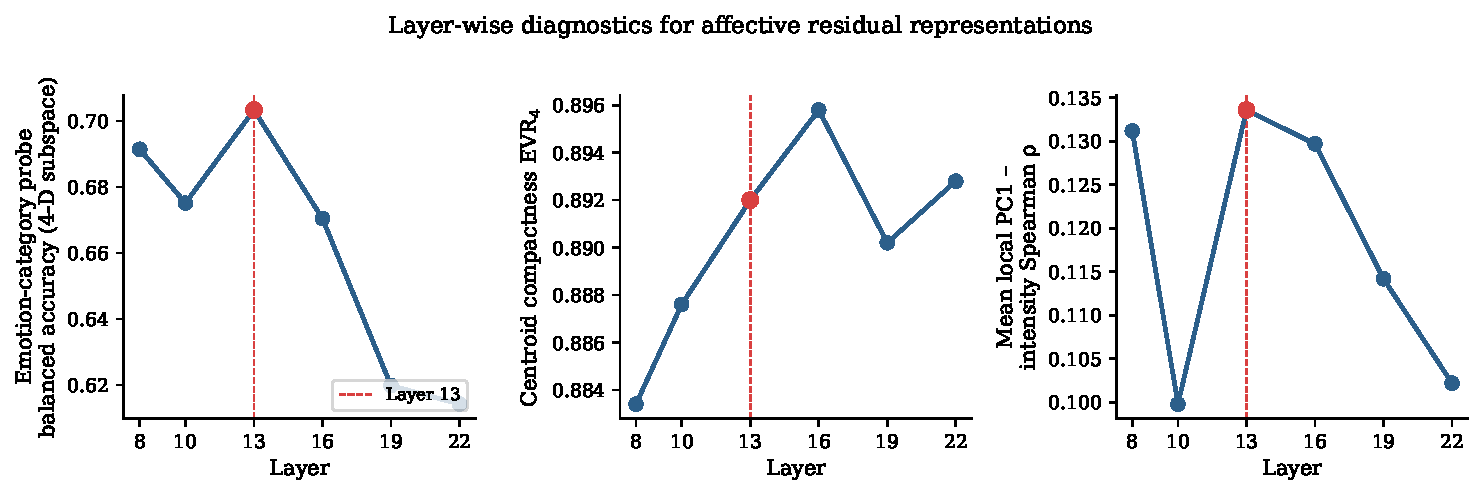
\includegraphics[width=0.8\linewidth]{figures/layer_diagnostics_lineplot.pdf}
    \caption{A visualisation of the layer diagnostics across candidate layers.}
    \label{fig:layer_diagnostics}
\end{figure}

First, emotion-category probe performance in the 4D affective subspace is highest at layer 13. The balanced accuracy reaches 0.7033 at layer 13, compared with 0.6751 at layer 10 and 0.6704 at layer 16. On this criterion, layer 13 preserves the most linearly decodable information about the target emotion categories.

Second, this increase in decodability does not come at the cost of geometric compactness. The centroid-level four-dimensional explained variance remains high at layer 13, with $\mathrm{EVR}_{4}=0.8920$. This is slightly below layer 16 ($\mathrm{EVR}_{4}=0.8958$) but above layer 10 ($\mathrm{EVR}_{4}=0.8876$). In other words, layer 13 is not the strongest layer on this metric alone, but it remains close to the best-performing depth while retaining stronger emotion-category separability.

Third, layer 13 shows the strongest sensitivity to graded affective variation among the candidate layers. The mean local PC1 intensity correlation is 0.1336 at layer 13, compared with 0.0998 at layer 10 and 0.1297 at layer 16. Although the absolute correlation is modest, the relative increase suggests that layer 13 is the most sensitive of the three candidate layers to systematic changes in affective intensity.

To avoid overfitting the analysis to a single depth, we also examined neighbouring layers as robustness checks. Layers 10 and 16 show similar qualitative trends and preserve the main geometric findings, suggesting that affective structure is not confined to a single transformer block. We therefore do not treat layer 13 as uniquely optimal in a global sense. Rather, we use it as the main reporting layer because it offers the best trade-off across the three diagnostics, while layers 10 and 16 serve as nearby robustness checks.

\section{Linear Probe Analysis}

% Present probes as the first decodability test.
% Separate category decodability from intensity decodability.
% Use this subsection to motivate why geometry and steering matter beyond simple classification.

\section{CAA Vector Construction}

% Explain how CAA directions are built from emotion vs neutral activations.
% Mention pooled directions across intensity levels if used.
% Frame these as candidate steering vectors.

\section{Latent Geometry of Emotion}

% Summarize what the geometry says about the representation space.
% Include participation ratio, explained variance, and cross-emotion similarity.
% Put local PCA or emotion-axis structure here if you want that material in the chapter.

\section{Steering Experiments}

% Describe alpha sweeps and what they test.
% Cover directionality, monotonicity, and content preservation.
% Include shift accuracy and robustness as evidence that the directions are causally useful.

\section{Limitations and Transition}

% State the main failure modes or unresolved issues.
The analyses in this chapter are intended to establish four claims: that CAA directions can be constructed from the emotion rewrite dataset, that emotion is reasonably well separated in a narrow band around layer 13, that the resulting space contains both common emotionalisation structure and emotion-specific residual structure, and that steering can satisfy directionality, approximate monotonicity, and partial semantic preservation. The next chapter turns these representational claims into an explicit evaluation protocol, covering controlled steering benchmarks and human-centred assessment.